\section*{Приёмы работы с элементами презентации}
\addcontentsline{toc}{section}{Приёмы работы с элементами презентации}
\subsection*{Движение между двумя ограниченными линиями}
\addcontentsline{toc}{subsection}{Движение между двумя ограниченными линиями}

\textbf{Задание:}\\
Реализовать в среде AnyLogic движение между двумя ограниченными линиями.\\

\textbf{Решение:}\\
Построим два параллельных отрезка и квадрат между ними. (Рисунок \ref{fig:rectangle1})
\begin{figure}[h]
	\centering 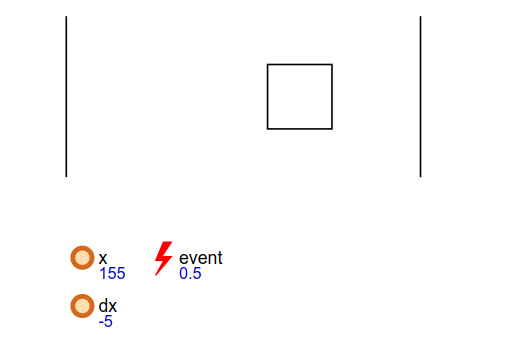
\includegraphics[scale=0.5]{rectangle1}
	\caption{Схема модели в AnyLogic}
	\label{fig:rectangle1}
\end{figure}

Для решения данной задачи нужно завести переменную $x$, которая будет отвечать за текущие координаты квадрата. Также потребуется переменная $dx$, которая отвечает за направление движения квадрата. В событии стоит прописать следующий код. (Рисунок \ref{fig:rectangle2})
\begin{figure}[h]
	\centering 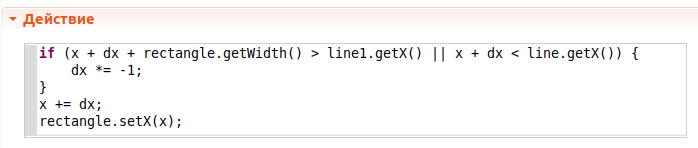
\includegraphics[scale=0.5]{rectangle2}
	\caption{Алгоритм события движения прямоугольника}
	\label{fig:rectangle2}
\end{figure}

Получается, что если мы дошли до границы второй линии или наоборот дошли до границы первой линии, то квадрат меняет своё направление движения. Также он стабильно наращивает свою позицию в соответствии с направлением и обновляет свои координаты.